Cette section détaille les couches évoquées dans l'autre section \ref{partie_architecture} et complète sur les paquetages \textit{factory} (visible sur la figure \ref{diagramme_de_paquetage_idb}) et \textit{useful}.

\subsection{Paquetage des fabriques}
L'application utilise une \textit{fabrique abstraite} qui se trouve dans le paquetage \textit{factory}.

\subsubsection{Utilité}
L'une des problématiques est de faire fonctionner l'application avec tous les SGBD disponibles.
Bien que le langage SQL soit normé, les SGBD ne l'implémentent pas de la même manière, ce qui veut dire que la syntaxe des requêtes est \underline{différente} d'un SGBD à l'autre.
Ce point constitue la difficulté principale du développement, et la fabrique abstraite permet de la régler tout en respectant les principes \textit{ouvert/fermé}. Elle permet également de régler d'autres problèmes mineurs, comme la gestion de la casse qui diffère d'un SGBD à l'autre
\footnote{\label{casse_et_sgbd}Oracle convertit le nom des tables et contraintes en majuscule, ce qui n'est pas le cas de MySQL par exemple.}.

En raison du temps disponible pour le développement, l'application ne fonctionne qu'avec les SGBD Oracle et MySQL.
En revanche, elle accueille un nouvel SGBD sans \textbf{modifier} le code existant: il faut seulement en \textbf{ajouter}. %pas de u après le e pour accueille

\subsubsection{Dépendances supplémentaires}
Les dépendances de ce paquetage ne sont pas toutes représentées sur la figure \ref{diagramme_de_paquetage_idb}.
Le diagramme montre que la fabrique est toujours appelée depuis un contrôleur (par le biais d'une façade).
En plus de cette dépendance, des dépendances de stéréotypes \textit{create} existent :
\begin{itemize}
\item vers le paquetage gui, pour que les IHM utilisent une stratégie de saisie différente en fonction du SGBD (gestion de la casse par exemple),
\item vers le paquetage manager, pour que le code SQL généré ait la syntaxe du SGBD connecté.
\end{itemize}

\subsubsection{Statique de la fabrique}
\begin{figure}[!h]
  \centering
  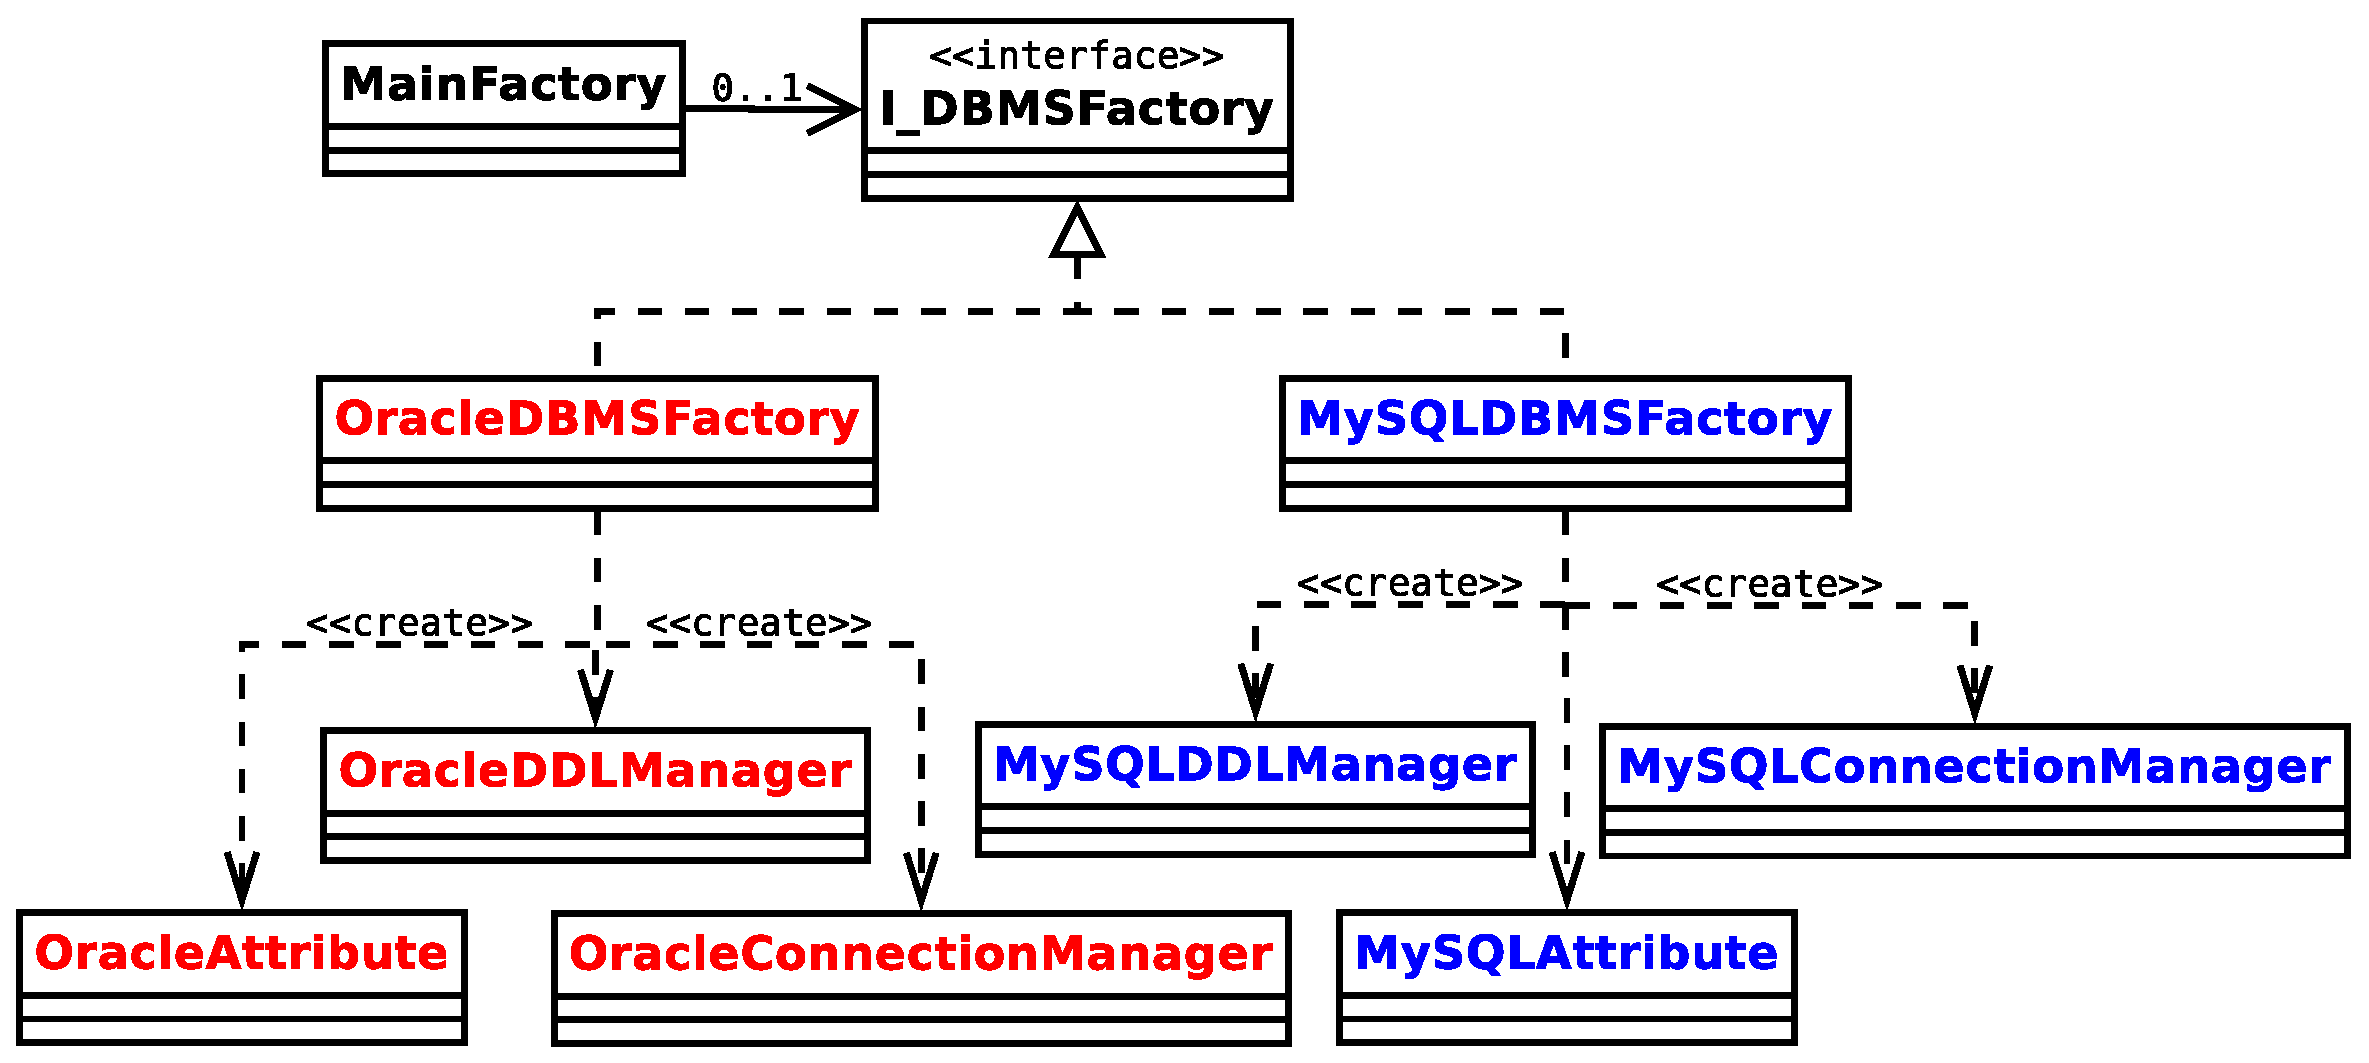
\includegraphics[width=14cm]{images/diagramme_classes_fabriques.eps}
  \caption{Fabrique abstraite de l'application. Génère des objets différents selon le SGBD connecté.}
  \label{diagramme_classes_fabrique}
\end{figure}

Sur la figure \ref{diagramme_classes_fabrique}, la classe \textit{MainFactory} est une fabrique concrète de fabriques abstraites.
Elle s'associe avec une \textit{I\_DBMSFactory} qui représente le SGBD connecté pour créer les bons objets, ce qui correspond à un pattern \textit{stratégie}.

La seule fabrique de l'application est MainFactory.
Pour ajouter un nouvel SGBD, il faut créer une classe qui implémente l'interface I\_DBMSFactory, donc \textbf{ajouter} du code.
La seule \textbf{modification} nécessaire se trouve dans MainFactory, pour qu'elle puisse instancier l'implémentation.

\subsection{Paquetage des outils}
Plusieurs classes sont utilisées un peu partout dans le code.
Ces classes (développées par l'équipe du projet) sont regroupées dans le paquetage \textit{useful}, qui n'apparaît pas sur la figure \ref{diagramme_de_paquetage_idb}.

\subsubsection{Dépendances}
Tous les paquetages de cette application dépendent du paquetage useful, mais ce n'est pas gênant dans la mesure où le code de ces classes n'est jamais amené à changer.
Ce paquetage peut être comparé à \textit{java.util}
\footnote{\label{paguetage_java_util}Package \textit{java.util} : \url{https://docs.oracle.com/javase/7/docs/api/java/util/package-summary.html}}
de java, qui contient les utilitaires que l'on retrouve dans toutes les applications.

\subsubsection{Classe Response}
\begin{figure}[!h]
  \centering
  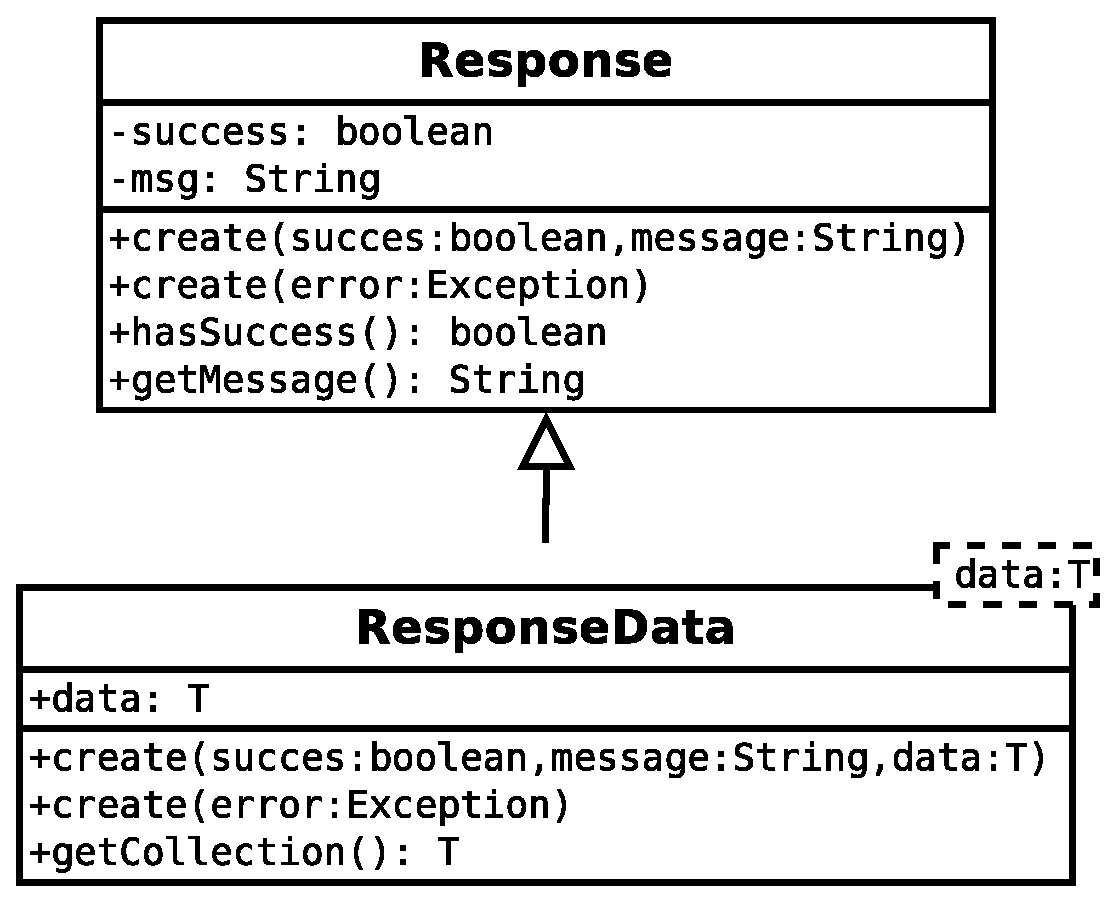
\includegraphics[width=10cm]{images/response.eps}
  \caption{La classe Response en mode plan.}
  \label{uml_classe_response}
\end{figure}

Les DAO de l'application utilisent les packages \textit{java.sql} et \textit{javax.sql}
\footnote{\label{paquetages_sql}Package \textit{java.sql} : \url{https://docs.oracle.com/javase/7/docs/api/java/sql/package-summary.html}}.
En cas de problèmes lors du dialogue avec les SGBD, les méthodes de ces packages lèvent les exceptions \textit{SQLException}.

Travailler avec les exceptions est pénible : elles forcent à utiliser des clauses \textit{try/catch} où à déclarer des méthodes qui lèvent des exceptions.
La programmation devient chaotique puisqu'elle se rapproche d'une programmation événementielle, la ligne d'exécution peut sauter à tout moment pour se retrouver dans la clause catch.
Il faut ensuite gérer les types de retour des méthodes ou les exceptions levées.

Dans ce projet, les exceptions restent bloquées dans les classes du paquetage manager.
Les méthodes retournent des objets \textit{Response} et ne lèvent aucune exception.

Cette classe possède deux attributs, comme le montre la figure \ref{uml_classe_response}:
\begin{enumerate}
\item un booléen, vrai si et seulement si la méthode du DAO a réussi,
\item une chaîne de caractère qui contient un message du SGBD si la méthode du DAO a échouée, ou un message de réussite si tout c'est bien passé.
\end{enumerate}

Avec Response, on récupère donc deux informations en un seul \textit{return}.
Les succès ou les échecs des appels au SGBD sont traités uniquement dans instructions conditionnelles.

Ces objets sont utilisés également dans les IHM : une Response dont le premier attribut est faux affiche un message rouge d'erreur.
Une Response positive affiche un message bleu.

\subsubsection{Classe ResponseData<T>}
La classe Response est spécialisée par ResponseData.
Elle est utile lorsque le DAO est utilisé pour \textbf{récupérer} des informations du SGBD.
En plus des informations de la classe Response, elle possède une collection d'objets T.
Elle peut par exemple stocker le résultat d'une requête SELECT ou encore retourner le nom des tables disponibles dans la base de données.

\subsection{Paquetage des IHM}
Les IHM sont regroupées dans le paquetage \textit{gui}.

\subsubsection{Diagramme de classes des IHM}
\begin{figure}[!h]
\centering
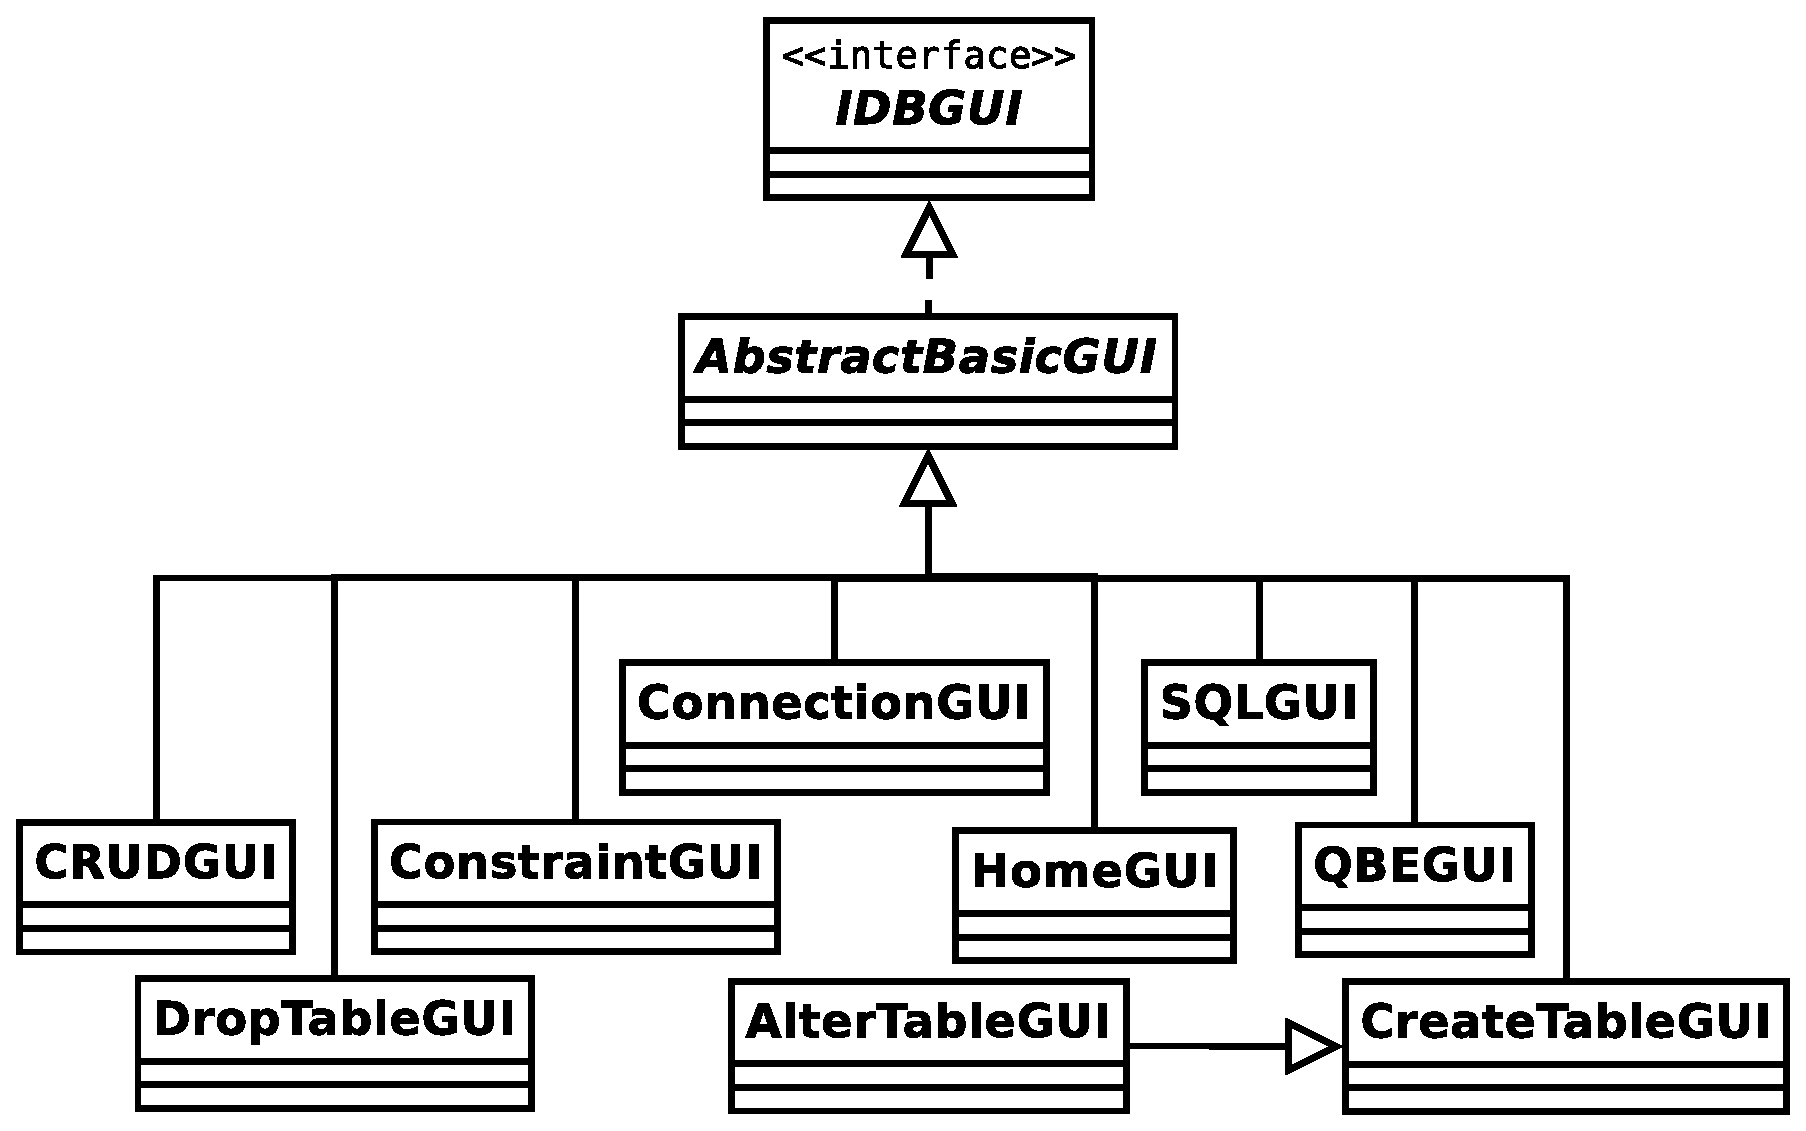
\includegraphics[width=14cm]{images/gui.eps}
\caption{Les IHM spécialisent \textit{AbstractBasicGUI}.}
\label{hierarchie_des_ihm}
\end{figure}

AbstractBasicGUI regroupe un ensemble de méthodes qui gèrent seules l'agencement des composants
\footnote{\label{composants_ihm}Barre de défilements, case à cocher, étiquettes, boite saisie etc.}
, ce qui permet de concevoir une IHM en se focalisant sur le fond plutôt que sur la forme.

\subsubsection{Comportement commun}
Les IHM utilisent les méthodes suivantes :
\begin{itemize}
\item \textit{talk()}, qui communique avec l'utilisateur en écrivant un message sur une étiquette située \textbf{en haut} de la fenêtre,
\item \textit{isComplete()}, qui autorise à appuyer sur le bouton "final" d'une IHM si et seulement si toutes les informations sont remplies.
\end{itemize}

En généralisant le comportement des IHM, l'utilisateur prend des habitudes sur l'application, ce qui la rend plus ergonomique.

\subsection{Paquetage des gestionnaires}
Le paquetage \textit{manager} regroupe les DAO et d'autres outils.
Tout le contenu n'est pas détaillé dans cette sous-section.

Les gestionnaires sont \textit{développés pour des interfaces} , afin de respecter le principe \textit{ouvert/fermé} et de permettre à l'application de se connecter à n'importe quel SGBD.
Les objets sont instanciés depuis la fabrique MainFactory.

\subsubsection{Gestionnaires de connexion}
Les méthodes de connexions varient d'un SGBD à l'autre avec le \gls{JDBC}.
Par conséquent, les classes qui gèrent la connexion implémentent une interface \textit{I\_ConnectionManager} (figure \ref{connection_managers_uml}.

\begin{figure}[!h]
\centering
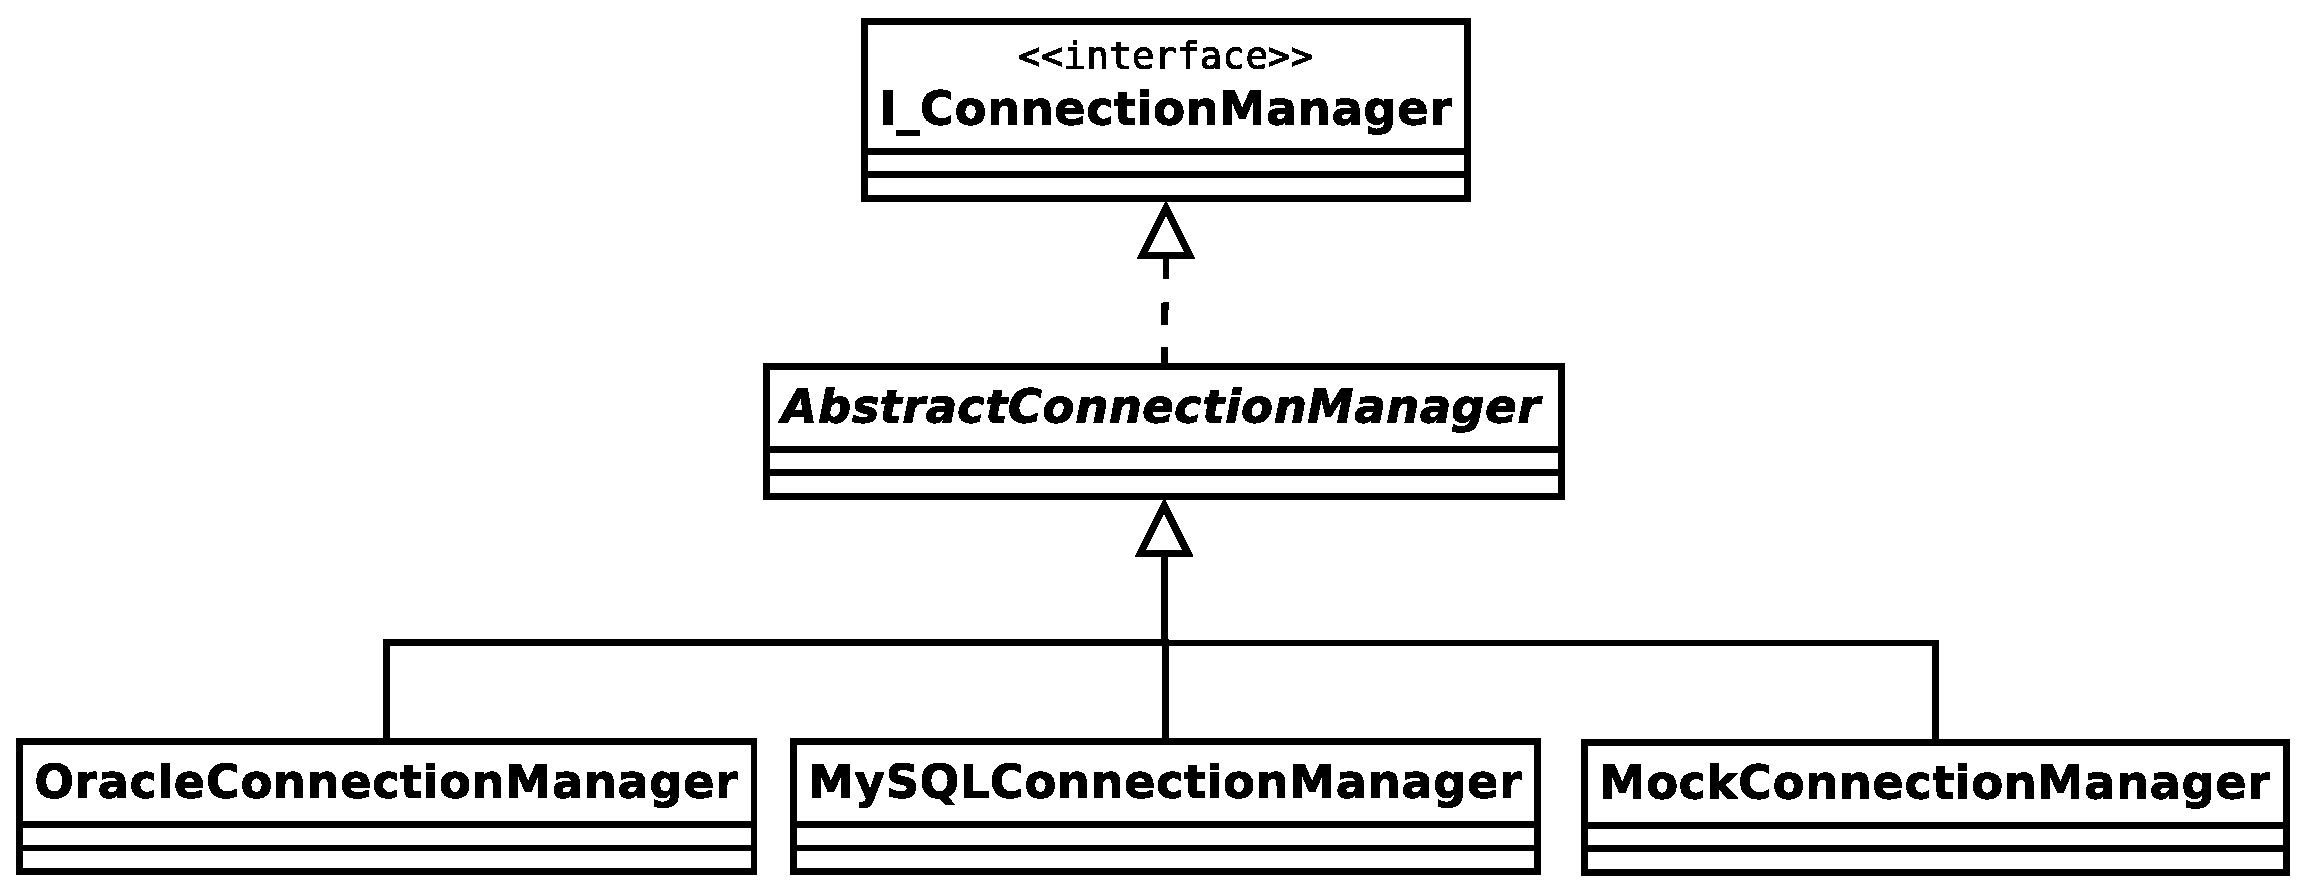
\includegraphics[width=14cm]{images/connection_managers.eps}
\caption{Implémentations du I\_ConnectionManager.}
\label{connection_managers_uml}
\end{figure}

\subsubsection{Gestionnaires de définition des données}
Les gestionnaires de définition des données sont développés pour une interface \textit{I\_DDLManager} afin de générer les requêtes SQL de LDD compatibles avec le SGBD connecté (figure \ref{ddl_managers_uml}).

\begin{figure}[H]
\centering
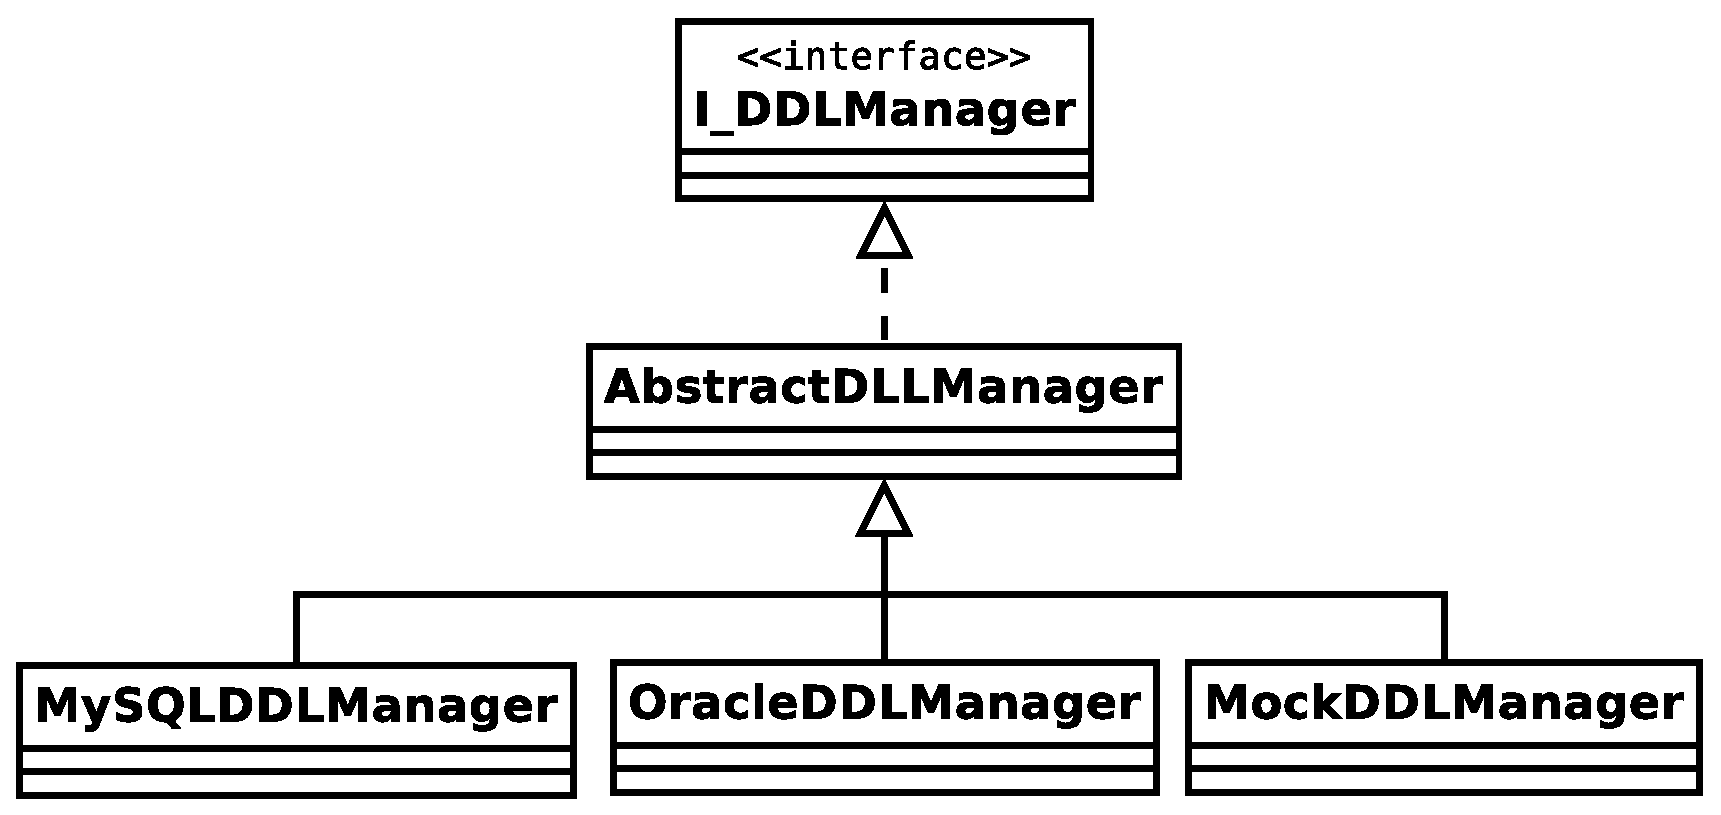
\includegraphics[width=14cm]{images/ddl_managers.eps}
\caption{Implémentations du I\_DDLManager}
\label{ddl_managers_uml}
\end{figure}
